\section{函数递归}
我们提及过,不只有主函数可以调用其它函数,任何函数都可以调用其它函数。我们也在先前的例子中看到,在 \lstinline@max(double,double,double)@ 中调用 \lstinline@max(double,double)@ 是完全可行的。那么一个函数能否调用它本身呢?C/C++给出的答案是可以。这种``一个函数调用它本身''的情况,在编程领域有一个专门的名字,叫作\textbf{递归(Recursion)}。\par
你可能会有困惑:我怎么能用一个东西来定义它本身呢?那不就成了逻辑学上的循环定义了?别急,且先听我慢慢道来。\par
数学上有个函数叫作阶乘(Factorial),对于非负整数$n$,它的定义是$n!=1\times2\times3\times\ldots\times n$(特殊定义$0!=1$)。它还有一种递推定义:$0!=1; n!=n\times(n-1)!$。\par
如何理解这个递推定义呢?其实就是,$0!$的值是给定的,而$n!$的值要由$n$乘以$(n-1)!$来计算。那么$(n-1)!$如何计算呢?要通过$n-1$乘以$(n-2)!$来计算。这样不断推导下去,就能一直推到$0!$这个确定的数据,因此只要知道了$0!$,就可以一步一步推出$n!$的值来。\par
而在编程当中,我们可以用函数递归的方法来计算阶乘,下面是一个示例代码:
\begin{lstlisting}[caption=\texttt{Factorial\_with\_Recursion.cpp},label=lst:FactorialWithRecursion]
//用递归方法实现阶乘函数
#include <iostream>
using namespace std;
//如果fractorial的参数大于12,就会发生运算结果溢出。可以考虑用unsigned long long
unsigned factorial(unsigned n) { //阶乘的参数和值都不是负数,所以定义成unsigned
    if (n == 0) { //终止条件,不可或缺
        return 1; //0!为1,直接返回
    }
    else { //如果没有到达终止条件,就调用factorial(n-1),离终止条件更近一步
        return n * factorial(n - 1); //递归,n!用n*(n-1)!表示
    }
}
int main() {
    cout << factorial(12); //计算并输出12!的值
    return 0;
}
\end{lstlisting}
我来解释一下这段代码,并回答一下读者可能关心的问题。\par
\textit{``我用 \lstinline@factorial@ 来定义 \lstinline@factorial@,编译器不会报错吗?''}\par
不会的,因为\textbf{函数的定义就是一种声明}。所以编译器在 \lstinline@factorial@ 函数给定参数列表时就已经知道了它的存在(图4.5)。\par
\begin{figure}[htbp]
    \centering
    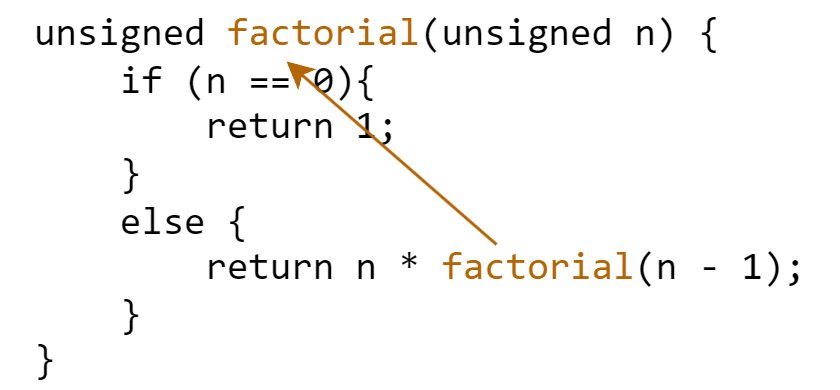
\includegraphics[width=0.5\textwidth]{../images/generalized_parts/04_factorial_code_logic_300.png}
    \caption{\lstinline@factorial@ 的定义就是一种声明,所以编译器能够找到它}
\end{figure}
\textit{``这段代码会怎么运行?''}\par
想像你就是那个程序,在主函数中,当你遇到 \lstinline@factorial(12)@ 时,你会调用这个函数并代入实参 \lstinline@n=12@ 从而求出它的返回值。而在运行时发现,因为 \lstinline@n==0@ 不满足,所以你不得不再去求 \lstinline@factorial(11)@,然后是 \lstinline@factorial(10)@,以此类推。如果一切顺利的话,你会在求 \lstinline@factorial(0)@ 的时候直接返回 \lstinline@1@,然后用 \lstinline@1*factorial(0)@ 算出 \lstinline@factorial(1)@ 的返回值;用 \lstinline@2*factorial(1)@ 算出 \lstinline@factorial(2)@ 的返回值;用 \lstinline@3*factorial(2)@ 算出 \lstinline@factorial(3)@ 的返回值……一直到你算出 \lstinline@factorial(12)@ 为止。图4.6展示了这一过程。\par
\begin{figure}[htbp]
    \centering
    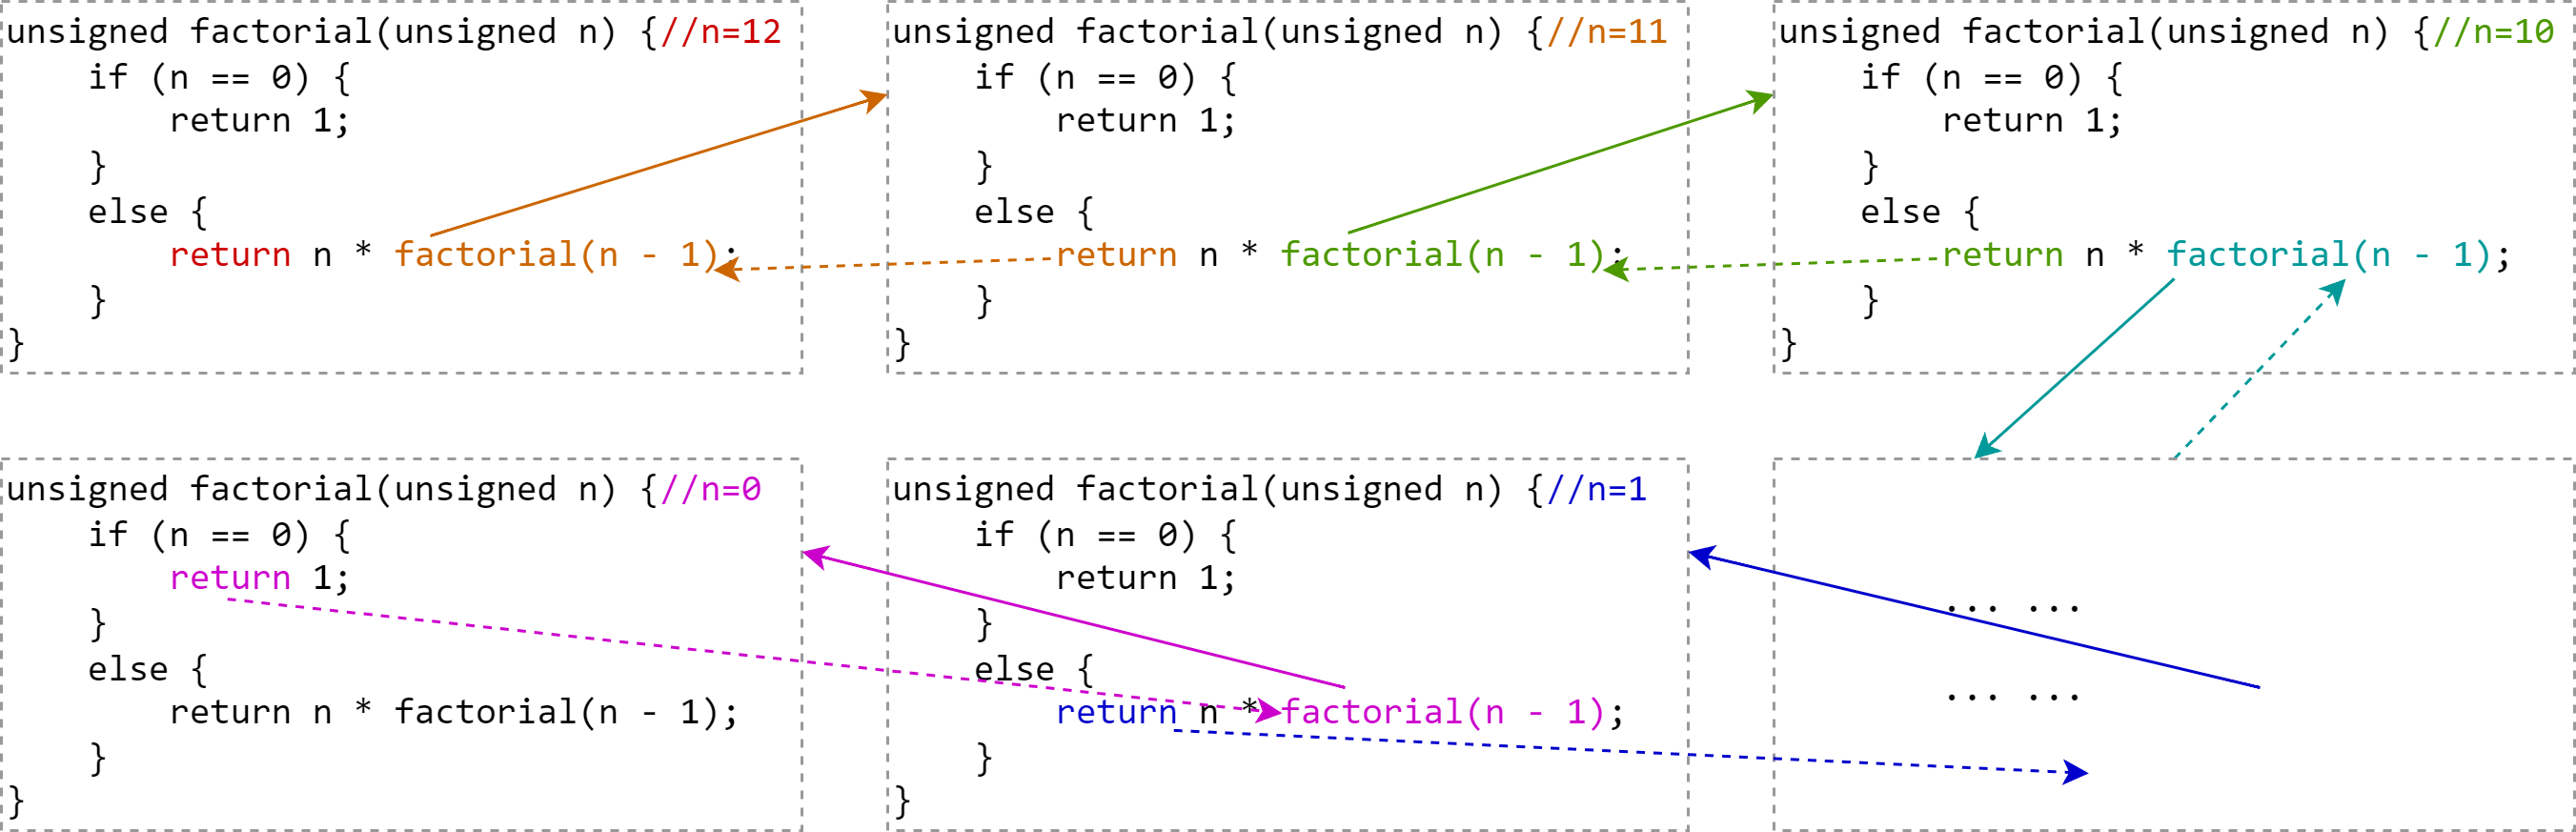
\includegraphics[width=\textwidth]{../images/generalized_parts/04_the_process_of_recursion_300.png}
    \caption{\lstinline@factorial@ 函数递归的运行过程}
\end{figure}
\textit{``函数递归运行的过程中,难道还能真的像图4.6那样,运行到一半再跑到开头吗?''}\par
读者可能容易产生这样的误会,认为``既然它是同一个函数,那递归的时候不就是在这一个函数中打转嘛''。\par
不然。这个函数在编译时和运行时的概念是不同的。在编译时,编译器会认为它是一个函数;但在运行时,内存中会为程序创建一个调用栈(Call stack)来存储函数调用的信息。每次函数调用(包括一般调用和递归调用)都会在栈中压入一个堆栈帧(Stack frame),这个堆栈帧中存储了本次调用的必要信息(比如,本次调用的实参是什么,返回地址是什么)。在结束调用时,返回值传回给调用它的函数(栈的结构保证了调用它的函数也在调用栈中),然后堆栈帧移除,如图4.7。\par
\begin{figure}[htbp]
    \centering
    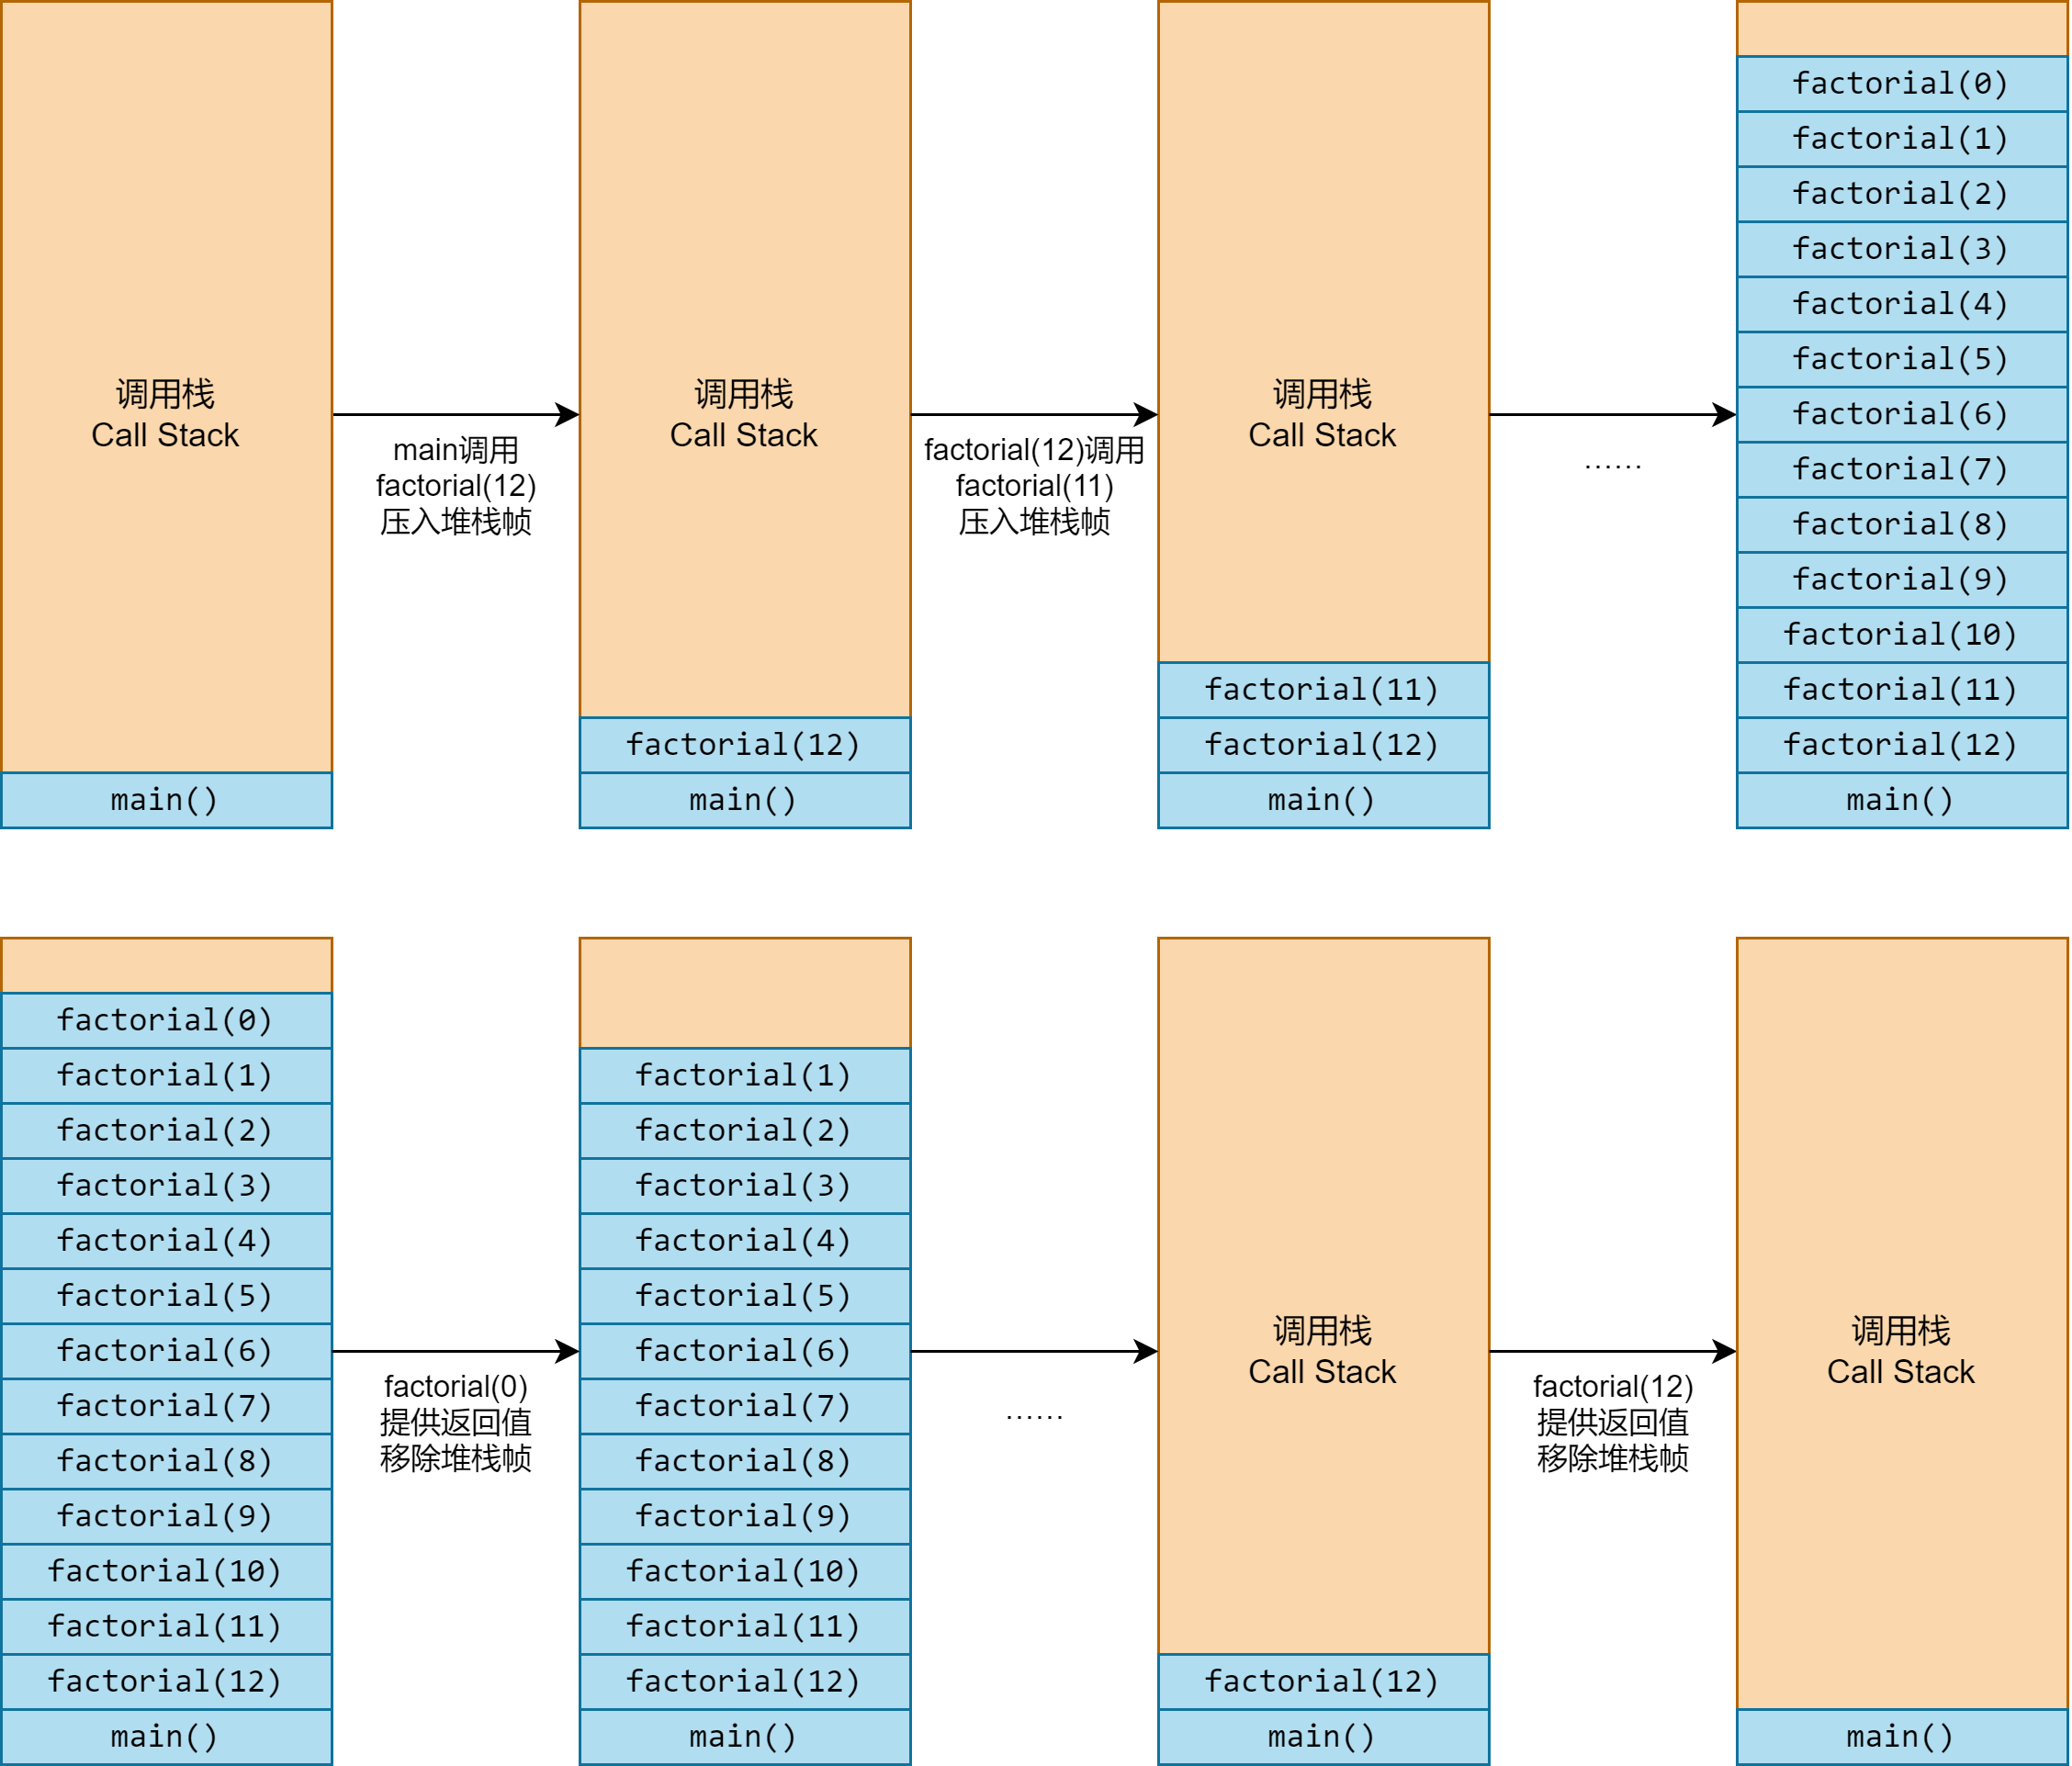
\includegraphics[width=0.8\textwidth]{.//images/generalized_parts/04_call_stack_structure_300.png}
    \caption{调用函数时压入堆栈帧,返回值后移除堆栈帧}    
\end{figure}
简言之,虽然\textbf{只有一个函数},但\textbf{有很多个堆栈帧},每个堆栈帧存储了各自的调用信息。所以自然不会有什么冲突了。\par
\textit{``为什么一定要有终止条件呢?难道不能像 \lstinline@while(true)@ 语句这样永远循环吗?''}\par
我们可以把递归结构当作是一种循环,而 \lstinline@for@ 或 \lstinline@while@ 可以更具体地说是一种迭代(Iteration)。从功能上讲,递归和迭代是非常相似的,它们可以互相替代,而关于``用递归还是迭代''的讨论也是旷日持久。这里我们先不参与此讨论,只解答原本的问题。\par
递归与迭代有一点不同在于,迭代语法不需要依赖调用栈,比如 \lstinline@for(int i=0;i<1e9;i++)@,无论循环多少次,\lstinline@i@永远占据一个 \lstinline@int@ 的内存空间;但递归是需要依赖调用栈的,并且调用栈的大小有限,一旦内存不够,就会发生\textbf{堆栈溢出(Stack overflow)},直接导致程序故障罢工。正因如此,我们可以写无限循环的迭代,但不能写一个无限循环的递归。\par
希望读者看过上述的讲解以后,已经对递归有了基本的认知。\par
在编程时,善用递归可以帮助我们节省很多写代码的麻烦。再举个例子,我们打算写一个简单的求斐波那契数\footnote{斐波那契数列(Fibonacci sequence),是一个特殊的数列。它的前两项都是1,而后面的每个斐波那契数都由前两数相加得到。前十个斐波那契数为:1, 1, 2, 3, 5, 8, 13, 21, 34, 55。}的函数,通过传入的正整数参数 \lstinline@n@ 来求出斐波那契数列的第 \lstinline@n@ 项。\par
如果用递归来写这个函数,就要比迭代轻松不少(尤其是在我们还没有学习数组的时候)。\par
\begin{lstlisting}
unsigned fibonacci(unsigned n) {
    if (n <= 2) { //前两个数的值都是1,直接给定
        return 1;
    }
    else { //第n个数由第n-2个数加第n-1个数得到
        return fibonacci(n - 2) + fibonacci(n - 1);
    }
}
\end{lstlisting}\par
